%% --------------------------------------------------------------
%% Academic Manuscript Template
%% WihanZA
%% wihanmarais@sun.ac.za
%% --------------------------------------------------------------

%% Document class
\documentclass[
12pt,
a4paper,
twoside,
]{article}

%% Language | Dates
\usepackage[main=british]{babel}
\usepackage[english]{isodate}
\cleanlookdateon

%% Margins | Spacing
\usepackage[left=1in, right=1in, top=1.2in, bottom=1.2in]{geometry}
\usepackage[skip, parfill, indent=1em]{parskip}
% default parskip is .5\baselineskip plus 2pt
\usepackage{setspace}
\setstretch{1}
\setlength{\emergencystretch}{3em}
\raggedbottom
\providecommand{\tightlist}{\setlength{\itemsep}{0pt}\setlength{\parskip}{0pt}}
\def\lineheight{16}
\usepackage{pdflscape}

%% Ignore badboxes of less than 3pt
\hfuzz=3pt

%% Math | Font
\usepackage{amsmath}
\usepackage{amssymb}
\usepackage[utf8]{inputenc}
\usepackage{textcomp}
\usepackage[vvarbb, upint, subscriptcorrection, uprightscript]{notomath}
\usepackage{noto-mono}
\usepackage[rmdefault]{sourceserifpro}
\usepackage[sfdefault]{sourcesanspro}
\usepackage[T1]{fontenc}
\renewcommand\familydefault{\rmdefault}
\usepackage[normalem]{ulem}
\usepackage{bm}
\let\bm\symbfit
\usepackage{fontawesome}

%% Microtypography
\usepackage[
protrusion=true,
factor=1000,
expansion=true,
auto=true,
verbose=true
]{microtype}

\DisableLigatures{encoding=T1,shape=sc}

%% Headings
\usepackage{titlesec}

% Section format
\titleformat{\section}
    {\sffamily\fontseries{sb}\scshape\Large\selectfont}
    {\thesection}
    {1ex}
    {}

% \titlespacing{\section}
%     {0pt}
%     {2ex plus 0.2ex minus .1ex}
%     {1.5ex plus 0.2ex minus .1ex}

% Unnumbered section format
\titleformat{name=\section,numberless}
    {\sffamily\fontseries{sb}\scshape\Large\selectfont}
    {}
    {0pt}
    {}

% Subsection format - smaller than section
\titleformat{\subsection}
    {\sffamily\fontseries{sb}\scshape\large\selectfont}
    {\thesubsection}
    {1ex}
    {}

% Subsubsection - even smaller for better hierarchy
\titleformat{\subsubsection}
    {\sffamily\fontseries{sb}\scshape\normalsize\selectfont}
    {\thesubsubsection}
    {1ex}
    {}

% Paragraph format
\titleformat{\paragraph}
    [runin]
    {\sffamily\fontseries{sb}\scshape\normalsize\selectfont}
    {}
    {0pt}
    {}
    [\quad]

%% Symbols
\usepackage{siunitx}
\sisetup{}
\sisetup{
detect-all = true,
detect-family = true,
output-decimal-marker = {.},
group-separator = {\,},
number-unit-product = {\,},
inter-unit-product = \mathord{\cdot},
exponent-product = \mathord{\times},
separate-uncertainty = true}

%% Packages
\usepackage{calc}
\usepackage{etoolbox}

%% Floats
\usepackage{float}
% figures only float within the sections they are defined in
\usepackage[section]{placeins}

%% Tables
\usepackage{array}
\usepackage{longtable}
\usepackage{booktabs}
\setlength{\tabcolsep}{6pt}
\renewcommand{\arraystretch}{1.25}
\usepackage{tabu}
\usepackage{threeparttable}
\usepackage{threeparttablex}
\usepackage{makecell}

%% Figures | Graphics
\usepackage{graphicx}
\usepackage{wrapfig}

%% Captions
\usepackage[font={footnotesize, singlespacing}]{caption}
\captionsetup[figure]{labelfont={bf},labelformat={default},labelsep=quad,name={Fig.}}
\captionsetup[table]{labelfont={bf},labelformat={default},labelsep=quad,name={Table}}

%% Code chunk printing

%% Lists
\usepackage{enumitem}

%% Metadata
\makeatletter
\providecommand{\subtitle}[1]{
\apptocmd{\@title}{\par {\large\textit{#1} \par}}{}{}
}
\makeatother
\title{My Manuscript}
\subtitle{A Template\footnote{Thanks to all the participants at the
  conference for their feedback.}}

\author{
Johnny E. Bravo%
\thanks{Corresponding author. Department of Economics, Hanna-Barbera
University.
\\ \faEnvelopeO \ \href{mailto:johnnybravo@gmail.com}{\nolinkurl{johnnybravo@gmail.com}}}
 \and %
Homer J. Simpson%
\thanks{Department of Economics, University of Springfield.
\\ \faEnvelopeO \ \href{mailto:homersimpson@yahoo.com}{\nolinkurl{homersimpson@yahoo.com}}}
}

\date{25 Apr 2025}

%% Customise \maketitle
\makeatletter
\def\@maketitle{%
  \newpage
  \null
  \vskip 1em%
  \begin{center}%
  \let \footnote \thanks
  {\LARGE \@title \par}%
    \vskip 1em%
  {\large \lineskip .5em%
  \begin{tabular}[t]{c}%
  \@author
    \end{tabular}\par}%
  \vskip 1em%
  % {\normalsize\sffamily\fontseries{sb}\scshape Version}\par\vspace{-.5em}
  {\normalsize \@date}%
  \end{center}%
  \par
  \vskip 1em}
\makeatother

%% Abstract
\makeatletter
\renewenvironment{abstract}{%
\if@twocolumn
    \section*{\abstractname}%
\else
    \normalsize
    \begin{center}%
      {\sffamily\fontseries{sb}\scshape \abstractname\vspace{-.5em}\vspace{\z@}}%
    \end{center}%
\fi}
\makeatother

%% Headers | Footers | Page numbers
\usepackage{fancyhdr}
% title page style is set to empty below
\pagestyle{plain}
\pagenumbering{arabic}

%% Footnotes
% setspace package must load before footmisc
\usepackage[hang, multiple]{footmisc}

% defaults
% \hangfootparskip =  0.5\baselineskip
% \hangfootparindent = 0em
% \footnotemargin = 1.8em

\renewcommand*{\hangfootparskip}{.5\baselineskip}
\renewcommand*{\hangfootparindent}{0em}
\renewcommand*{\footnotemargin}{1em}

%% make title page footnotes same as rest
\makeatletter
\patchcmd\maketitle{\@makefntext}{\@@@ddt}{}{}
\patchcmd\maketitle{\rlap}{\mbox}{}{}
\makeatother

%% Color
\usepackage[table,dvipsnames]{xcolor}
\definecolor{stbWine}{rgb}{0.65, 0.04, 0.24}

%% URLs
\usepackage[hyphens]{url}
\urlstyle{same}

%% Hyperref
\usepackage[unicode]{hyperref}
\hypersetup{breaklinks=true,
            pdftitle={My Manuscript},
            pdfauthor={},
            colorlinks=true,
            filecolor={teal},
            linkcolor={teal},
            citecolor={teal},
            urlcolor={teal},
            pdfborder={0 0 0}}

%% Bibliography
\usepackage[round, nonamebreak]{natbib}
\bibliographystyle{plainnat}
\renewcommand{\bibsection}{\section*{\refname}\pdfbookmark{References}{sec:references}}
\renewcommand\bibfont{\small}

%% Acronyms
\usepackage{acronym}
\acrodef{ppml}[PPML]{poisson pseudo-maximum likelihood}
\acrodef{ols}[OLS]{ordinary least squares}
\acrodef{mno}[MNO]{mobile network operator}
\acrodef{ma}[M\&A]{mergers and acquisitions}

%% Cross-referencing
\usepackage[capitalize,noabbrev]{cleveref}

%% Subfigures
\usepackage[labelformat=simple,labelfont=sf]{subcaption}

%% Fix cross-referencing for subfigures
\renewcommand\thesubfigure{(\alph{subfigure})}
\makeatletter
\renewcommand\p@subfigure{\thefigure\space} % prefix used in \ref and \cref for subfigures
\makeatother

%% Fix problem with amsmath cleveref acronym
%% https://github.com/WihanZA/wihantemplates/issues/2
%% https://tex.stackexchange.com/a/735502
\makeatletter
    \AtBeginDocument
    {
      \def\ltx@label#1{\cref@label{#1}}
      \def\label@in@display@noarg#1{\cref@old@label@in@display{#1}}
    }
\makeatother

%% Adapted from %% https://tex.stackexchange.com/questions/71364/acronym-acresetall-cleveref-multiply-defined-labels
%% Add \AC before @verridelabel
\makeatletter
\newcommand*{\org@overidelabel}{}
\let\org@overridelabel\AC@verridelabel
\renewcommand*{\AC@verridelabel}[1]{%
  \@bsphack
  \protected@write\@auxout{}{\string\AC@undonewlabel{#1@cref}}%
  \org@overridelabel{#1}%
  \@esphack
}%
\makeatother

%% Line numbering
%% Load after amsmath because of conflict
%% https://github.com/latex-lineno/lineno/issues/5

%% Header includes
\usepackage{booktabs}
\usepackage{longtable}
\usepackage{array}
\usepackage{multirow}
\usepackage{wrapfig}
\usepackage{float}
\usepackage{colortbl}
\usepackage{pdflscape}
\usepackage{tabu}
\usepackage{threeparttable}
\usepackage{threeparttablex}
\usepackage[normalem]{ulem}
\usepackage{makecell}
\usepackage{xcolor}

%% Document
\begin{document}

%% Include before

\maketitle

%% no headers and page numbers in the title page
\thispagestyle{empty}

\begin{abstract}
  \quotation
  \small \selectfont \noindent Amet ultricies etiam nunc, dui a natoque
massa taciti ut id! Erat nec venenatis magna, leo libero ut augue
mollis. Curae orci, blandit lectus: vivamus potenti auctor quisque
dapibus auctor leo. Dui eleifend iaculis pellentesque malesuada placerat
lectus egestas -- cum nullam. Vitae mi consequat mollis nisi facilisis
posuere natoque volutpat. Dolor fringilla placerat non, quisque dictumst
-- ridiculus posuere egestas felis. Erat integer porttitor pretium purus
et sed ante duis torquent. Sagittis montes neque faucibus, pulvinar
penatibus mi scelerisque potenti; curabitur inceptos id urna. Congue
ultrices tortor lobortis suspendisse, tortor a, mollis facilisi? Fusce
potenti turpis eleifend accumsan cursus suscipit nunc rhoncus semper
tristique?
      \vspace{1ex}
  \begin{description}[font=\sffamily\fontseries{sb}\scshape, itemsep=1ex]
    \item[JEL Classification:]  C78  \( \cdot \)  D86  \( \cdot \)  L14 
    \item[Keywords:]  Keyword 1  \( \cdot \)  Keyword
2  \( \cdot \)  Keyword 3 
  \end{description}
      \endquotation
\end{abstract}


\clearpage

\section{Introduction}\label{introduction}

Lorem molestie scelerisque sodales ullamcorper, tortor, quis cum duis
ligula auctor. Eget volutpat pretium augue montes inceptos eros urna
convallis nullam pharetra. Dignissim convallis purus, blandit, mattis
convallis tempor ridiculus at felis nam. Laoreet curae cum fames sociis
dapibus rutrum mattis! Velit pretium odio, vehicula, ornare odio, lacus
dapibus feugiat. Eu torquent magna potenti et etiam purus luctus augue
sollicitudin? Augue iaculis congue odio montes at, integer himenaeos a
accumsan purus orci quam tempus, cum felis scelerisque.

Lorem iaculis sodales cursus ornare, velit vel mollis. Metus enim enim
ridiculus imperdiet venenatis fusce bibendum sociis eros pulvinar quam?

Adipiscing eleifend tellus, turpis nam accumsan, nam massa? Enim
dictumst porttitor malesuada, maecenas auctor sapien gravida pharetra
phasellus. Class ultrices senectus ullamcorper magna montes neque
inceptos semper quisque turpis eget tellus faucibus turpis

\subsection{Subsection heading}\label{subsection-heading}

Consectetur senectus tempor ornare semper commodo aenean a venenatis
torquent pellentesque ad. Condimentum mauris dui, ultrices vehicula
posuere placerat est nascetur quam. Vitae erat ultrices; et tempus
turpis morbi magna elementum. Nascetur et cubilia; natoque fames
interdum nec.

Consectetur diam ut porttitor ante ad nec placerat. Massa taciti conubia
pulvinar tempor tortor nullam ante nunc, curabitur ac sed. Velit at
sociis odio consequat sem facilisis eleifend ligula nam facilisi.
Maecenas nam cum justo habitant, quis euismod ad enim quis. Suspendisse
dictumst enim nunc.

Lorem nibh: scelerisque eleifend potenti cursus mi, vitae urna. Turpis
pulvinar suspendisse commodo nunc primis, eu libero tortor vehicula.
Faucibus ridiculus donec velit pharetra nibh mi, potenti, integer
feugiat nulla egestas. Nascetur nullam suscipit sollicitudin, non
vulputate primis nisl semper: varius nascetur netus nec? Gravida
tincidunt proin nibh facilisis imperdiet mi egestas lobortis iaculis.
Tortor vehicula dis fermentum a dis

\subsubsection{Subsubsection heading}\label{subsubsection-heading}

Amet blandit lectus rutrum libero accumsan fames ad. Eget fringilla
donec magnis metus augue auctor proin ornare. Mus mauris, morbi class
viverra augue hendrerit facilisis. Sociosqu nullam porttitor nec cras
vitae ullamcorper blandit, tempor vestibulum neque egestas dui ante?

Amet ut urna risus lacinia ante etiam tempus hendrerit. Est elementum
facilisi malesuada, ad dictum dui curae massa felis! Lacus fermentum
ridiculus vulputate bibendum in, fames erat iaculis lacus suspendisse
semper ad sollicitudin nam.

Adipiscing hendrerit nibh quam auctor vehicula, mi nec magna congue,
viverra inceptos? Porta dictumst sociis taciti vestibulum urna faucibus
quam porta laoreet dapibus molestie. Ultrices nostra malesuada class ac,
ligula at tempus conubia ornare felis. Euismod pulvinar dictum magna
commodo auctor cubilia tellus! Integer ut ligula, ultrices mus penatibus
commodo penatibus. Vivamus commodo tempor nec cubilia maecenas senectus

\paragraph{Paragraph heading}\label{paragraph-heading}

Consectetur tempus habitasse fames eu vitae, curae malesuada potenti
mus. Himenaeos urna etiam aptent metus eleifend dapibus ornare. Velit
fusce himenaeos -- blandit dictum dis dignissim habitasse. Quisque
quisque orci tristique posuere: vitae tristique varius, sed turpis nisi.
Dignissim netus?

Sit blandit velit viverra, gravida, lacus, imperdiet mus sem mollis!
Accumsan mi arcu tempus non mollis eleifend habitasse. Potenti euismod
risus accumsan convallis, diam: himenaeos tortor nam lobortis dui. Dui
laoreet cum primis facilisi elementum: facilisi laoreet, ut senectus,
torquent phasellus mauris enim. Cum morbi ad, urna nec aenean platea,
dapibus maecenas ultricies rutrum! Sodales leo hac donec pretium cum
rhoncus, parturient senectus nibh.

Adipiscing quisque et ut dapibus: leo molestie bibendum non torquent
varius. Facilisis fringilla ut per mus himenaeos ornare malesuada
feugiat curabitur? Sollicitudin consequat litora quam ullamcorper;
convallis donec vestibulum dis, ligula fermentum quis ante. Lacinia hac
posuere vestibulum libero; malesuada urna magna donec ad malesuada.
Venenatis vehicula parturient: fermentum facilisi, turpis -- quisque
scelerisque bibendum?

\section{Basics}\label{basics}

\subsection{Footnotes}\label{footnotes}

Footnotes are inserted using \texttt{\textbackslash{}footnote\{\}} in
LaTeX or \texttt{\^{}{[}{]}} in Markdown. See this example.\footnote{This
  is an example of a footnote.} Footnotes can also be managed with
\texttt{\textbackslash{}footnotemark} (or \texttt{{[}\^{}1{]}}) and
\texttt{\textbackslash{}footnotetext} (or \texttt{{[}\^{}1{]}:\ Text})
for more control over their placement and numbering. Here is a long
footnote.\footnote{Sit taciti tempus mollis cubilia, luctus nullam vel potenti morbi posuere magnis. Torquent proin volutpat porttitor, sociis eget facilisis et. Sapien non netus vivamus quam tempor fringilla rhoncus, pulvinar ad tortor. Praesent laoreet ultrices inceptos elementum nisl porta ultrices facilisi.

Adipiscing suspendisse egestas praesent aptent dui dui mi litora parturient. Eleifend ante morbi risus aliquam orci maecenas. Sociosqu aliquet laoreet curae sed ad mus, mauris – ut posuere at; congue inceptos ultricies. Magna hac nam ac id facilisi, condimentum rutrum himenaeos aliquet.

Ipsum purus nisl per cursus ante. Mollis cras sollicitudin aliquet sed eleifend ullamcorper pulvinar mauris aenean! Netus magna dui leo dictum pulvinar enim pellentesque urna. Iaculis rhoncus mollis euismod donec sapien interdum varius penatibus sociis tempus eget fames placerat felis ullamcorper faucibus}

\subsection{LaTeX sizes}\label{latex-sizes}

\begin{itemize}
\tightlist
\item
  \texttt{\textbackslash{}baselineskip}: \the\baselineskip
\item
  \texttt{\textbackslash{}smallskipamount}: \the\smallskipamount
\item
  \texttt{\textbackslash{}medskipamount}: \the\medskipamount
\item
  \texttt{\textbackslash{}bigskipamount}: \the\bigskipamount
\item
  \texttt{\textbackslash{}1em}: \the\fontdimen6\font
\item
  \texttt{\textbackslash{}1ex}: \the\fontdimen5\font
\end{itemize}

\subsection{Lists}\label{lists}

Itemized lists can be created using Markdown syntax like this:

\begin{itemize}
\tightlist
\item
  Item 1
\item
  Item 2
\item
  Item 3
\end{itemize}

Numbered lists can be created using Markdown syntax like this:

\begin{enumerate}
\def\labelenumi{\arabic{enumi}.}
\tightlist
\item
  Item 1
\item
  Item 2
\item
  Item 3
\end{enumerate}

These are equivalent to using the LaTeX environments \texttt{itemize}
and \texttt{enumerate}.

\subsection{Equations}\label{equations}

\def\bE{\mathbf{E}}
\def\bB{\mathbf{B}}
\def\bJ{\mathbf{J}}
\def\bx{\mathbf{x}}
\def\by{\mathbf{y}}
\def\bv{\mathbf{v}}
\def\bp{\mathbf{p}}
\def\bxdot{\mathbf{\dot x}}
\def\bal{\boldsymbol{\alpha}}
\def\bphi{\boldsymbol{\varphi}}
\def\e{\varepsilon}

\textbf{An inversion formula:} Let \(g:\mathbb{R}^+\to \mathbb{R}\) be
bounded and right continuous, and let
\(\varphi(\alpha)\coloneq\int_0^\infty e^{-\alpha t}g(t)\,dt\) denote
its Laplace transform. Then, for every \(t>0\), \begin{equation}
g(t)=\lim_{\mathstrut\varepsilon\to 0}\lim_{\mathstrut\lambda\to\infty}\varepsilon^{-1}\sum_{\lambda t<k\le (\lambda+\varepsilon)t}
\frac{(-1)^k}{k!}\lambda^k\varphi ^{(k)}(\lambda).\label{eq:inversion}
\end{equation}

\textbf{Solutions of systems of ODEs:} Let
\(\mathbf{v}(\mathbf{x},\boldsymbol{\alpha})\) denote a parametrized
vector field (\(\mathbf{x}\in U\), \(\boldsymbol{\alpha}\in A\)) where
\(U\) is a domain in \(\mathbb{R}^n\) and the parameter space \(A\) is a
domain in \(\mathbb{R}^m\). We assume that \(\mathbf{v}\) is
\(C^k\)-differentiable as a function
of\textasciitilde{}\((\mathbf{x},\boldsymbol{\alpha})\),
where\textasciitilde{}\(k\ge 2\). Consider a system of differential
equations in\textasciitilde{}\(U\): \begin{equation}
\mathbf{\dot x}=\mathbf{v}(\mathbf{x},\boldsymbol{\alpha}),\qquad \mathbf{x}\in U\label{eq:first}
\end{equation} Fix an initial point \(\mathbf{p}_0\) in the interior of
\(U\), and assume
\(\mathbf{v}(\mathbf{p}_0,\boldsymbol{\alpha}_0)\neq\mathbf{0}\). Then,
for sufficiently small \(t\), \(|\mathbf{p}-\mathbf{p}_0|\) and
\(|\boldsymbol{\alpha}-\boldsymbol{\alpha}_0|\), the
system\textasciitilde(\ref{eq:first}) has a unique solution
\(\mathbf{x}_{\boldsymbol{\alpha}}(t)\) satisfying the initial condition
\(\mathbf{x}_{\boldsymbol{\alpha}}(0)=\mathbf{p}\), and that solution
depends differentiably (of class\textasciitilde{}\(C^k\)) on \(t\),
\(\mathbf{p}\) and \(\boldsymbol{\alpha}\).

\textbf{Maxwell's equations:} \begin{equation*}
\begin{aligned}
\mathbf{B}'&=-c\nabla\times\mathbf{E}\\
\mathbf{E}'&=c\nabla\times\mathbf{B}-4\pi \mathbf{J}.
\end{aligned}
\end{equation*}

\textbf{Residue theorem:} Let \(f\) be analytic in the region \(G\)
except for the isolated singularities \(a_1\), \(a_2\), \ldots, \(a_m\).
If \(\gamma\) is a closed rectifiable curve in \(G\) which does not pass
through any of the points \(a_k\) and if \(\gamma\approx 0\) in \(G\),
then
\[\frac{1}{2\pi i}\int_\gamma f=\sum_{k=1}^m n(\gamma;a_k)\,\mathrm{Res}(f;a_k).\]

\textbf{Maximum modulus principle:} Let \(G\) be a bounded open set in
\(\mathbb{C}\) and suppose that \(f\) is a continuous function on
\(\bar G\) which is analytic in \(G\). Then
\[\max \{|f(z)| : z\in \bar G\}=\max\{|f(z)| : z\in \partial G\}.\]

\subsection{Figures}\label{figures}

\begin{figure}[htbp]

{\centering 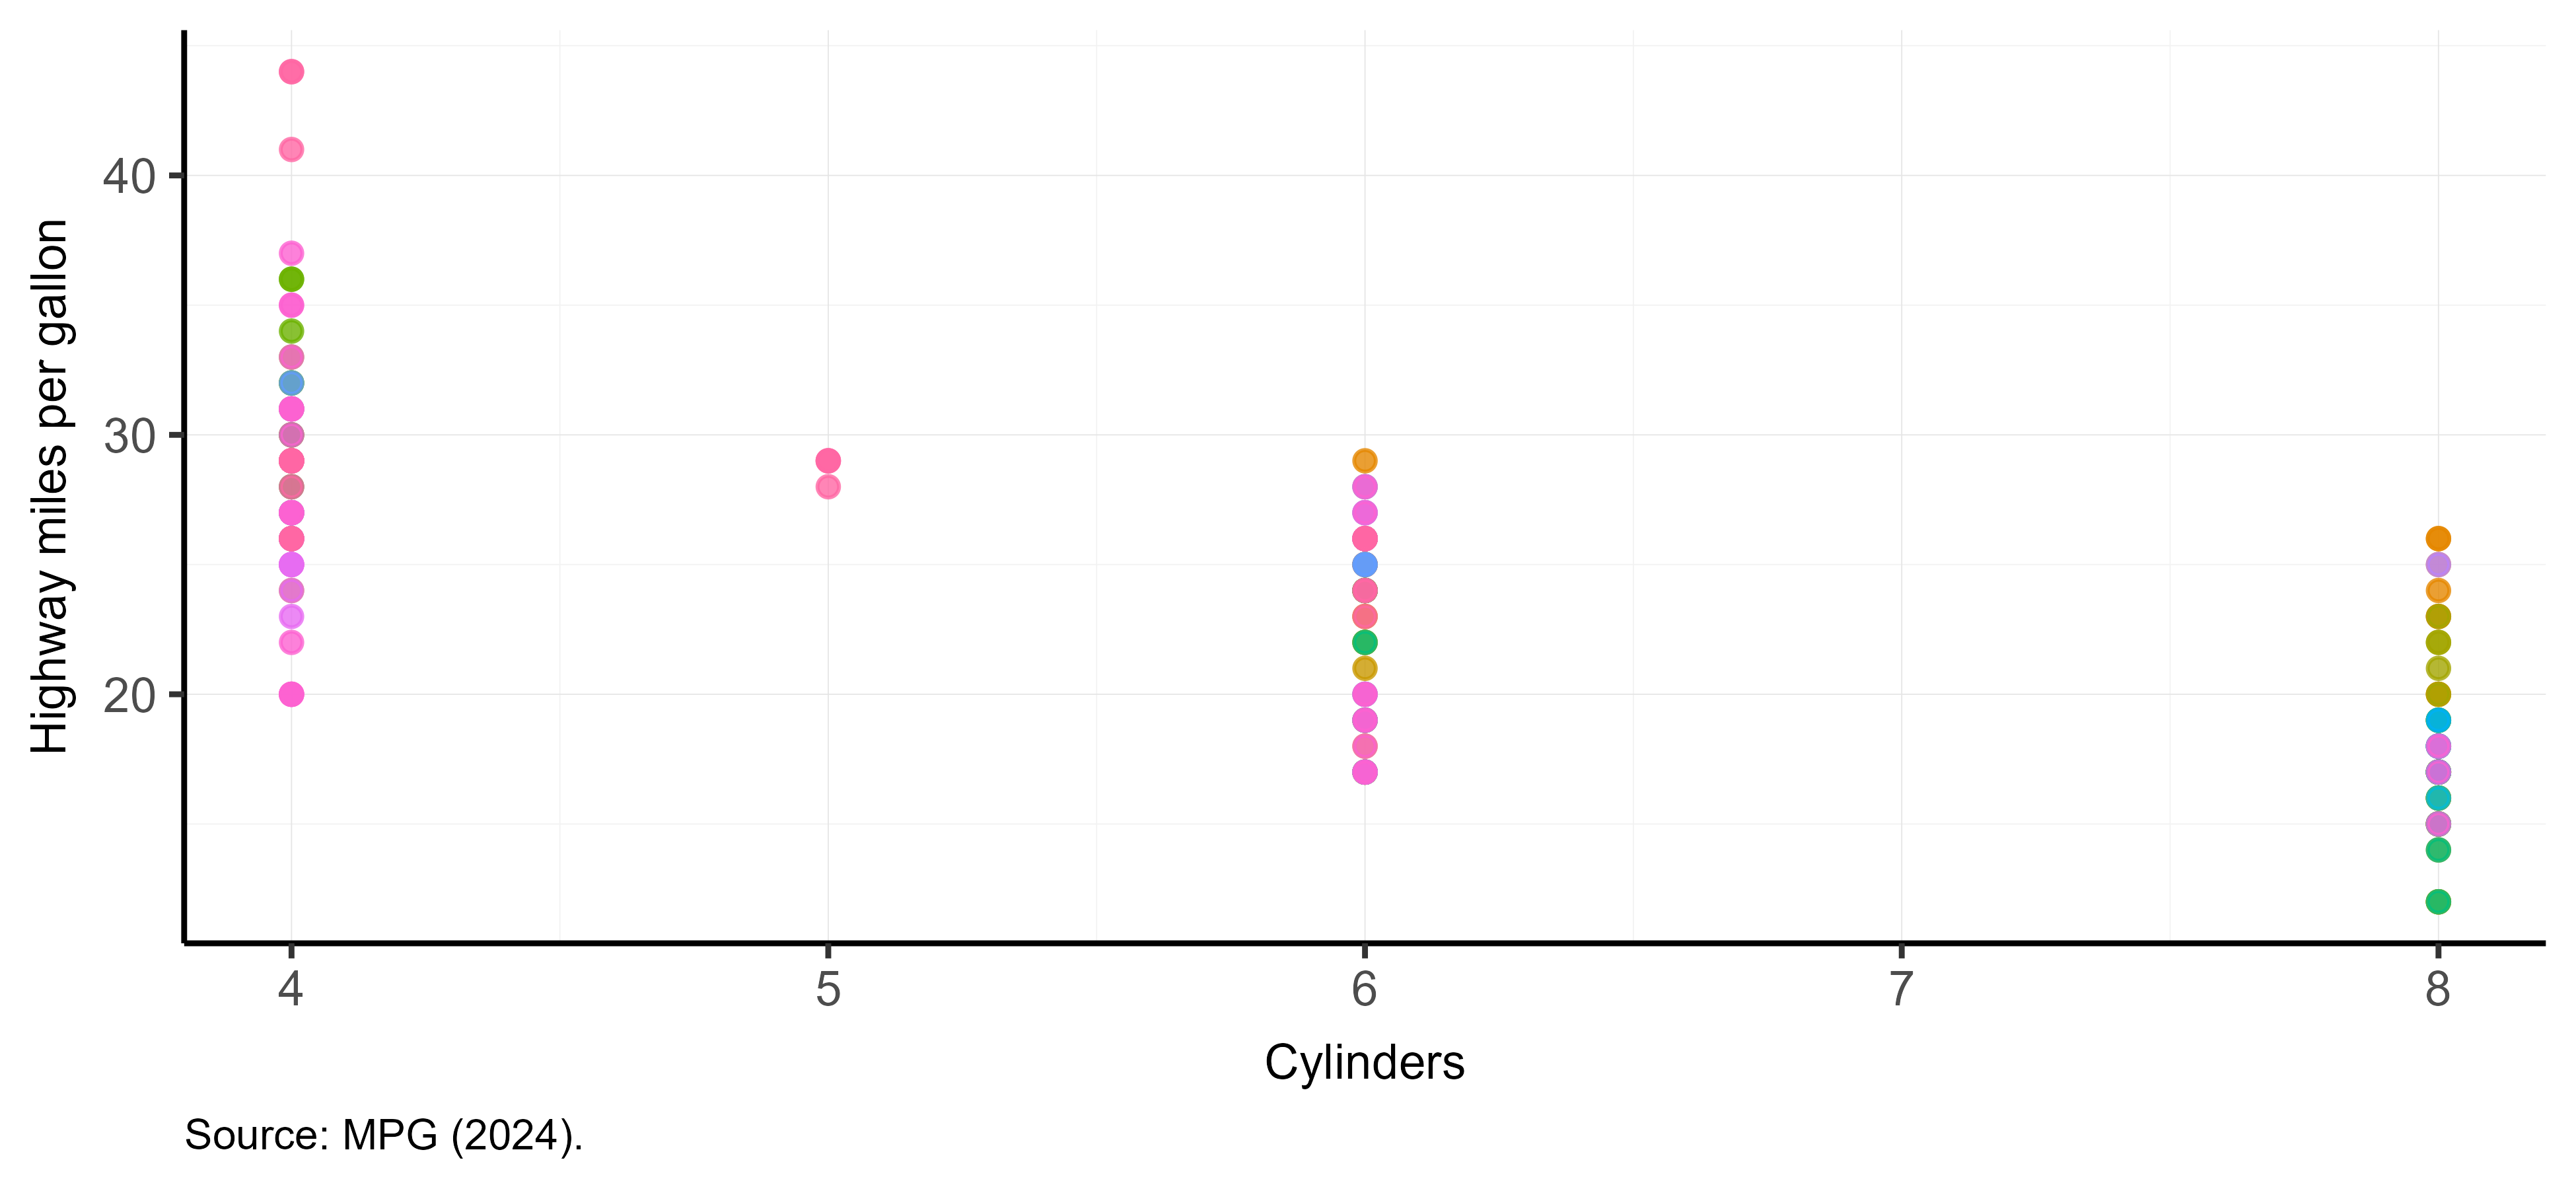
\includegraphics[width=0.95\textwidth]{figures/fancyplot} 

}

\caption{Manufacturer fuel efficiency}\label{fig:fancyplot}
\end{figure}

\subsection{Tables}\label{tables}

\begin{table}[H]
\centering
\caption{\label{tab:tab1}Caption centered above table}
\centering
\fontsize{10}{12}\selectfont
\begin{threeparttable}
\begin{tabular}[t]{lrrrr}
\toprule
  & mpg & cyl & disp & hp\\
\midrule
Mazda RX4 & 21.0 & 6 & 160 & 110\\
Mazda RX4 Wag & 21.0 & 6 & 160 & 110\\
Datsun 710 & 22.8 & 4 & 108 & 93\\
Hornet 4 Drive & 21.4 & 6 & 258 & 110\\
Hornet Sportabout & 18.7 & 8 & 360 & 175\\
Valiant & 18.1 & 6 & 225 & 105\\
\bottomrule
\end{tabular}
\begin{tablenotes}[para]
\item \textit{My footnote:} 
\item This is my table footnote.
\end{tablenotes}
\end{threeparttable}
\end{table}

\subsection{Acronyms}\label{acronyms}

\begin{itemize}
\tightlist
\item
  \texttt{\textbackslash{}ac\{ppml\}} produces ``\ac{ppml}'' the first
  time, and ``\ac{ppml}'' thereafter.
\item
  \texttt{\textbackslash{}acs\{ols\}} produces the short form
  ``\acs{ols}'' every time.
\item
  \texttt{\textbackslash{}acl\{ols\}} produces the long form
  ``\acl{ols}'' every time.
\item
  \texttt{\textbackslash{}acf\{ols\}} produces the full form
  ``\acf{ols}'' every time.
\item
  Plural forms are produced by adding \texttt{p} to the command, e.g.,
  \texttt{\textbackslash{}acp\{mno\}} for \acp{mno}.
\item
  Capitalization is produced by capitalizing the \texttt{A} of the
  command. For example, \texttt{\textbackslash{}Acl\{ppml\}} produces
  ``\Acl{ppml}''.
\item
  When defining acronym with key \texttt{ma}, remember to use slash
  (\texttt{\textbackslash{}}) to escape the ampersand (\&) in ``M\&A''
  so that \texttt{\textbackslash{}acs\{ma\}} produces \ac{ma}.
\end{itemize}

\subsection{Citations}\label{citations}

\begin{itemize}
\item
  \texttt{\textbackslash{}citet\{key\}} for textual citations like
  ``\citet{anderson_etal16}''.
\item
  \texttt{\textbackslash{}citet*\{key\}} expands to list all authors
  like ``\citet*{anderson_etal16}''.
\item
  \texttt{\textbackslash{}citep\{key\}} for parenthetical citations like
  ``\citep{anderson_etal16}''.
\item
  \texttt{\textbackslash{}citep*\{key\}} for a full author list like
  ``\citep*{anderson_etal16}''.
\item
  \texttt{\textbackslash{}citeauthor\{key\}} and
  \texttt{\textbackslash{}citeyear\{key\}}
  (\texttt{\textbackslash{}citeyearpar\{key\}}) cite the author(s) or
  year (in parentheses), respectively like:

  \begin{itemize}
  \tightlist
  \item
    ``\citeauthor{anderson_vanwincoop03}''
  \item
    ``\citeyear{anderson_vanwincoop03}''
  \item
    ``\citeyearpar{anderson_vanwincoop03}''
  \end{itemize}
\item
  Markdown offers similar functionality:

  \begin{itemize}
  \tightlist
  \item
    \texttt{@key} for textual citations and
  \item
    \texttt{{[}@key{]}} for parenthetical citations.
  \item
    \texttt{-@key} cites just the year.
  \end{itemize}
\item
  Mutliple citations can be combined using
  \texttt{\textbackslash{}citep\{key1,key2\}} like
  ``\citep{anderson_etal16, anderson_vanwincoop03}''.
\item
  Where possible, common elements in multiple citations are merged:

  \begin{itemize}
  \tightlist
  \item
    \texttt{\textbackslash{}citet\{fudd2020,\ fudd2021\}} produces
    ``\citet{fudd2020, fudd2021}''
  \item
    \texttt{\textbackslash{}citep\{fudd2020,\ fudd2020b\}} produces
    ``\citep{fudd2020, fudd2020b}''.
  \end{itemize}
\end{itemize}

\subsection{Cross-referencing}\label{cross-referencing}

\begin{itemize}
\tightlist
\item
  \texttt{\textbackslash{}label\{key\}} marks a target location.
\item
  \texttt{\textbackslash{}ref\{key\}} retrieves a basic reference.
\item
  \texttt{\textbackslash{}cref\{key\}} offers context-dependent
  referencing, adapting to the type of the referenced object.
\item
  \texttt{\textbackslash{}notag} is used to suppress the numbering of a
  line of an equation.
\end{itemize}

\begin{table}[H]
\caption{Cross-referencing commands and their outputs}
\label{tab:references}
\centering
\fontsize{10}{12}\selectfont
\begin{tabular}{@{}llll@{}}
\toprule
\texttt{key} & \texttt{\textbackslash ref\{key\}} & \texttt{\textbackslash cref\{key\}} & \texttt{\textbackslash eqref\{key\}} \\
\midrule
\texttt{fig:fancyplot} & \ref{fig:fancyplot} & \cref{fig:fancyplot} & - \\
\texttt{tab:tab1} & \ref{tab:tab1} & \cref{tab:tab1} & - \\
\texttt{eq:inversion} & \ref{eq:inversion} & \cref{eq:inversion} & \eqref{eq:inversion} \\
\texttt{equations} & \ref{equations} & \cref{equations} & - \\
\bottomrule
\end{tabular}
\end{table}

\section{Conclusion}\label{conclusion}

Sit turpis felis facilisis senectus lacus, phasellus risus torquent sed!
Vel suspendisse velit vivamus ornare justo suscipit velit ligula
elementum. Fringilla netus magnis nostra curae parturient lobortis: per
convallis bibendum. Lobortis habitasse netus mattis vel ultricies
suspendisse praesent ultricies, bibendum gravida.

Adipiscing lobortis placerat, aliquet; lobortis turpis erat; leo
ullamcorper himenaeos lacus hendrerit donec. Pharetra ut; sollicitudin
nec duis, habitant praesent, augue eros proin. Vulputate ligula porta
sem sagittis volutpat vel; consequat velit lacus. Quis ultricies magna
mus ligula?

Sit turpis facilisi nisi viverra: vestibulum magna arcu. Tempor cum
auctor mattis urna ac, condimentum hac curae nulla morbi. Faucibus
interdum non pulvinar; leo sodales facilisis volutpat? Varius luctus
penatibus proin litora ullamcorper auctor. Gravida sociis nec euismod
est tellus tempor diam dapibus sapien -- ridiculus habitasse primis.

Elit tristique est magnis, libero, taciti vulputate conubia magnis
inceptos platea. Interdum etiam elementum, porta litora condimentum
tellus orci sagittis nunc vitae. Congue porta nascetur cum curabitur
senectus, ullamcorper accumsan ut.

Consectetur primis mi phasellus phasellus nisi fringilla -- facilisis
tortor tempus id vivamus. A a etiam dui?

Sit fringilla dui cubilia suscipit feugiat ridiculus! Pulvinar tempor
potenti cras morbi cubilia facilisi vestibulum lobortis aliquet! Erat
purus, viverra aptent sollicitudin libero: feugiat, magnis laoreet
ornare phasellus. Sociis suscipit conubia torquent nec lobortis,
vestibulum luctus ultrices platea porttitor. Na porttitor.

Elit ridiculus a fames nunc cras pulvinar lectus vitae nisl. Vitae
pellentesque senectus nec feugiat nulla, risus eget placerat. Diam
suscipit, ante accumsan condimentum eleifend ut montes himenaeos duis
dignissim. Facilisis sociosqu egestas blandit nam feugiat eget metus
duis facilisi. Bibendum bibendum dapibus enim condimentum duis
tristique. Quis phasellus habitasse turpis nunc accumsan: platea
hendrerit -- volutpat eu lobortis a inceptos elementum rhoncus, torquent
-- morbi vehicula auctor inceptos blandit class.

Dolor diam velit vestibulum nostra eu -- netus egestas magnis cubilia
sollicitudin. Ligula malesuada orci nam netus, fermentum hendrerit?
Vestibulum integer per magna sollicitudin proin cursus, litora quam
donec neque euismod. Primis etiam habitasse mattis eget quisque eros,
egestas auctor mollis. Praesent sociis eget integer dictum sed? Justo
aliquam in sociosqu eros iaculis vehicula risus; justo risus commodo!
Netus fames dapibus mauris, vehicula dapibus cum porttitor nisl.
Hendrerit platea lobortis sodales maecenas aliquam eget diam donec
accumsan, habitasse donec vestibulum venenatis quisque himenaeos?

\clearpage

\bibliography{resources/mybib.bib}

%% Include after

\end{document}
